
\documentclass{acm_proc_article-me}

\usepackage[none]{hyphenat}
\sloppy

\begin{document}
\conferenceinfo{\textit{MediaEval 2014 Workshop,}}{October 16-17, 2014, Barcelona, Spain}

\title{Reordering the image search results for relevance and diversity in MediaEval 2014 Challenge}

\numberofauthors{3}

\author{
\alignauthor
Zsombor Par\'oczi\\
       \affaddr{Inter-University Centre for Telecommunications and Informatics}\\
       \email{paroczi@tmit.bme.hu}
\alignauthor
B\'alint Fodor\\
       \affaddr{Inter-University Centre for Telecommunications and Informatics}\\
       \email{balint.fodor@aut.bme.hu}
\alignauthor
G\'abor Sz\H ucs \\
       \affaddr{Inter-University Centre for Telecommunications and Informatics}\\
       \email{szucs@tmit.bme.hu}
}

\maketitle
\begin{abstract}
TODO abstract
\end{abstract}

\section{Introduction}

Many potential tourists do websearches when they try to find more information about a place he (or she) is potentially visiting. These people have only a vague idea about the location, knowing the name of the place. Our aim is to help them by providing a set of photos, as summary of the different views of the location. 
In the official challenge (Retrieving Diverse Social Images at MediaEval 2014: Challenge, Dataset and Evaluation) \cite{ionescu2014retrieving} a ranked list of location photos retrieved from Flickr (using text information) is given, and the task is, to refine the results by providing a set of images that are both relevant and provide a diversified summary. The diversity means that images can illustrate different views of the location at different times of the day/year and under different weather conditions, creative views, etc. The refinement and diversification process can be based on the social metadata associated with the collected photos in the data set~\cite{ionescu2014div400} and/or on the visual characteristics of the images. The initial results are typically noisy and redundant because of social media platform~\cite{radu2014hybrid}, where the large variety comes from very different users. 

The goodness of the refinement process can be measured using the precision and diversity metric~\cite{Taneva:2010:GRP:1718487.1718541}. Earlier we have solved a very similar problem by diversification of initial results using clustering~\cite{szHucs2013bmemtm}, but our solution was focused on diversification only. The largest development of this paper is that we focus on both the relevance and diversity.

\section{Reordering System}

We took five approaches to generate the final reordering of the inital search result. This required five different systems that share similar components. All the systems take the inital ordering as the input along with the visual feature descriptors and the textual descriptors corresponding to the images. In each case the relevancy of all images are estimated, the images are grouped into clusters and based on this two type of information the final ordering is determined.

Table \ref{table:runs}. shows the different system compositions we used. Section \ref{sec:relevance}. describes the 'average' ('avg') relevance estimation and its extended versions utilizing user credibility information. User credibilities are used with different weights in the last two approaches. Section \ref{sec:clust}. defines the methods we used to cluster the data.

\begin{table}[h]
\centering
\begin{tabular}{|c|c|c|}
	\hline 
	run name & relevance & clustering\tabularnewline
	\hline 
	\hline 
	run1 & avg & visual\tabularnewline
	\hline 
	run2 & avg & textual\tabularnewline
	\hline 
	run3 & avg & visual+textual\tabularnewline
	\hline 
	run4 & avg + credibility 1 & visual+textual\tabularnewline
	\hline 
	run5 & avg + credibility 2 & visual+textual\tabularnewline
	\hline 
\end{tabular}
\caption{Reordering approaches.}
\label{table:runs}
\end{table}

\subsection{Relevance Scoring}
\label{sec:relevance}

For every $k$th place in the orderings of the developer data set we calculated the probability of the item at the $k$th place is relevant. Before giving the formal definition let denote the set of all orderings in the developer set as $L$, the $k$th element of the ordering $l \in L$ as $l_k$ and the binary function of the relevancy (based on the ground truth data) as $r_{gt}(l_k)$. Then $p_k$, the estimated probability of the $k$th element in an ordering is relevant:
$p_k = \frac{1}{|L|}\sum_{l \in L}r_{gt}(l_k)$.

When processing an ordering (from the test data set) we give the relevance score of $p_k$ to the $k$th element of the ordering.

In table \ref{table:runs}. 'avg + credibility' means that the relevance estimation is multiplied by the user credibility (in range $[0,1]$). 

\subsection{Clustering}
\label{sec:clust}

The provided data sets contains visual feature descriptors (color moments, histogram of oriented gradients, etc.) in csv files. First, we merged the descriptors into a long feature vector, one vector for each image. The clustering is done per ordering, so the feature vector is calculated for every image in an ordering. Then the components of the vectors are normalized to bring all the data to the same scale. The vectors are clustered with the K-means algorithm by trying all clustering number parameters from 6 to 18. For every clustering the silhouette score~\cite{rousseeuw1987silhouettes} is calculated and the best instance is selected.

Clusterings based on textual and visual data can differ, but merging the two results can be beneficial. Having two clustering functions $c_1(x)$ and $c_2(x)$ that are mapping an image id to a cluster label, one can construct $c_3(x) = (c_1(x), c_2(x))$ that maps an image id to a new cluster labeled by the pair of the two original cluster labels. Note that the new label set is the Cartesian product of the two original cluster label sets.

\subsection{Final Ordering}

Our reordering algorithm (in order to get maximal $F_1$ value in each subset of the answer list) consists of four phases.

1) Take the elements in each cluster in descending order and select the element that possessing the largest probabilities of relevance, this will be the 1st in the reordered list.
2) $L$th step: take the first elements in each cluster as candidate and calculate the estimated $F_1$ measure: $$F_1(@L) = \frac{2 \cdot P(@L) \cdot CR(@L)}{P(@L) + CR(@L)}$$
3) Select the element possessing the largest estimated $F_1$ measure and move to the reordered list.
4) Continue with phase 2 until we have cluster elements left.

\section{Results and Conclusion}

Figures \ref{fig:p}., \ref{fig:cr}., \ref{fig:f1}. shows the values of P@N, CR@N and F1@N for the different runs, while table \ref{table:results}. shows the average P@20, CR@20 and F1@20 results.



\begin{table}[h]
\centering
\begin{tabular}{|l|r|r|r|}
	\hline 
	run name & P@20 & CR@20 & F1@20\tabularnewline
	\hline 
	\hline 
	run1 & .7602 & .4107 & .5259\tabularnewline
	\hline 
	run2 & .7809 & .4065 & .527\tabularnewline
	\hline 
	run3 & .7756 & .4127 & .5305\tabularnewline
	\hline 
	run4 & .7415 & .3651 & .4819\tabularnewline
	\hline 
	run5 & .7431 & .3682 & .4866\tabularnewline
	\hline 
\end{tabular}
\caption{Average results of the five approaches}
\label{table:results}
\end{table}

\begin{figure}[h]
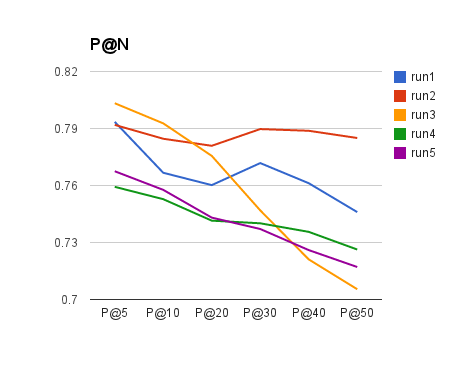
\includegraphics[width=0.9\linewidth]{p}
\caption{P@N results}
\label{fig:p}
\end{figure}

\begin{figure}[h]
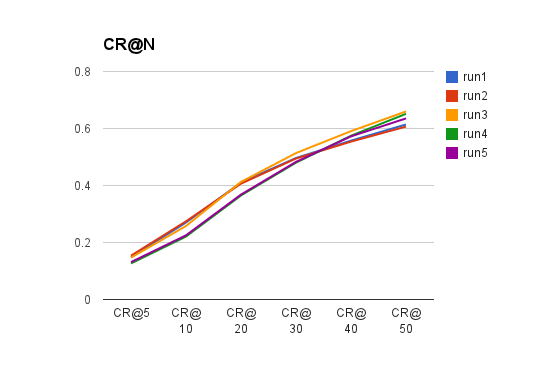
\includegraphics[width=0.9\linewidth]{cr}
\caption{CR@N results}
\label{fig:cr}
\end{figure}

\begin{figure}[h]
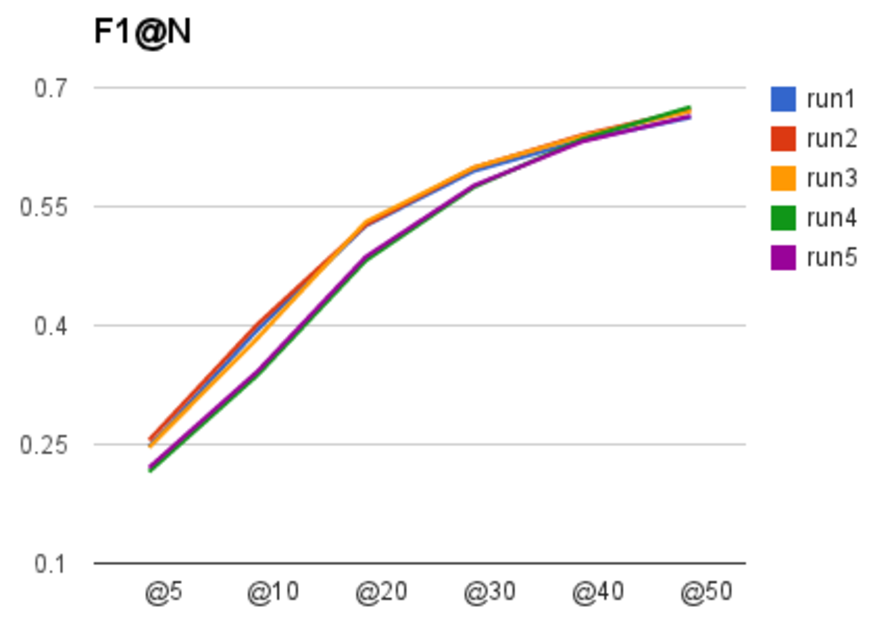
\includegraphics[width=0.9\linewidth]{f1}
\caption{F1@N results}
\label{fig:f1}
\end{figure}

\section{Acknowledgments}

The publication was supported by the T\'AMOP-4.2.2.C-11/1/KONV-2012-0001 project. The project has been supported by the European Union, co-financed by the European Social Fund.

\bibliographystyle{abbrv}
\bibliography{sigproc}

\end{document}
